% Benötigt: \usepackage{booktabs,array,amsmath,tikz}
% Zielzustand = Fail-closed-Politik und dreiwertiges Verdikt. Siehe Kommentare "CODE:" für Abweichungen vom aktuellen Repo.

\section{Requirements}
\label{sec:requirements}

This chapter derives the requirements for the verifier from the ProoVer 2026 task and from the properties of TSTP derivations discussed in Chapter~\ref{sec:background}.
Section~\ref{subsec:req-context} fixes the task and its assumptions.
Section~\ref{subsec:req-scoring} analyses the scoring scheme, which determines how the verifier should behave when it is unsure.
Sections~\ref{subsec:req-functional} and~\ref{subsec:req-nonfunctional} list the functional and non-functional requirements.
Section~\ref{subsec:req-traceability} relates them to the components and tests of the implementation.

\subsection{Task and Assumptions}
\label{subsec:req-context}

The verifier receives a FOF problem file and a TSTP proof file and must decide whether the proof is a valid refutation of the negated conjecture, i.e.\ a derivation of \texttt{\$false} from the axioms and the negated conjecture \citep{proover-competition}.
The proofs use the roles \texttt{axiom}, \texttt{conjecture}, \texttt{negated\_conjecture}, and \texttt{plain} and the statuses \texttt{thm}, \texttt{esa}, and \texttt{cth}.
A part of the benchmark proofs contains deliberate, subtle errors.
Only a small number of rules is specified by the organizers: Skolemization, the negated conjecture, and the import of axioms and conjectures.
All other steps may be checked by an external ATP, but only if they have status \texttt{thm} or \texttt{cth} and only with the step's premises.
The organizers state that handling edge cases is part of the task.

Let $P$ be a problem with axioms $A$ and conjecture $C$, and let a proof $\pi$ be a finite list of annotated formulas.
The verifier must decide whether $\pi$ is a \emph{valid refutation} of $P$:
(i) every \texttt{axiom} and \texttt{conjecture} step of $\pi$ is faithful to $P$;
(ii) the dependency graph of $\pi$ is acyclic and $C$ is used only by the step that negates it;
(iii) every other step is sound in the sense of Section~\ref{subsec:proof-objects-soundness}; and
(iv) $\pi$ derives \texttt{\$false}.
It answers \emph{verified}, \emph{failed}, or \emph{uncertain}.
The competition input is restricted to FOF; CNF and typed or higher-order input are out of scope.
We make the following assumptions:

\begin{itemize}
  \item The input files are syntactically close to the TPTP BNF, but may be large (thousands of steps) and deeply nested.
  \item The problem file is trusted, the proof file is not.
  \item An external ATP and a model finder may or may not be available at run time; the verifier must behave safely in both cases.
\end{itemize}

\subsection{Scoring and Its Consequences}
\label{subsec:req-scoring}

In ProoVer 2026 a correct rejection of an invalid proof scores $+2$, a correct acceptance of a valid proof $+1$, giving up $0$, a wrong rejection $-1$, and a wrong acceptance $-10$ \citep{PLACEHOLDER_PROOVER_PROC}.
Ties are broken by the average time on solved problems.
The asymmetry has a direct consequence for the verifier's behavior in uncertain situations.
Let $p$ be the probability that a given proof is valid, given everything the verifier has found out.
The expected scores of the three possible answers are
\begin{align*}
  E[\text{accept}] &= p\cdot 1 + (1-p)\cdot(-10) = 11p - 10,\\
  E[\text{reject}] &= p\cdot(-1) + (1-p)\cdot 2 = 2 - 3p,\\
  E[\text{abstain}] &= 0.
\end{align*}
Accepting is thus better than abstaining only if $p > 10/11 \approx 0.91$, and rejecting is better than abstaining only if $p < 2/3$.
For $2/3 < p < 10/11$, giving up is optimal.
The verifier therefore must not guess: it accepts only if every step has been positively verified, it rejects only if it has found a concrete defect, and it abstains in all other cases, for example if a required tool is missing or a time limit is hit.
A failed rule-specific check counts as a concrete defect only for rules without an ATP fallback; otherwise the step stays unresolved until the fallback has decided (Section~\ref{subsec:design-atp}).
Figure~\ref{fig:expected-score} visualizes the three expected scores.
The probability $p$ is of course not observable; the analysis does not compute it but motivates the asymmetric thresholds and the fail-closed policy that gives rise to the soundness requirement below.

\begin{figure}[t]
\centering
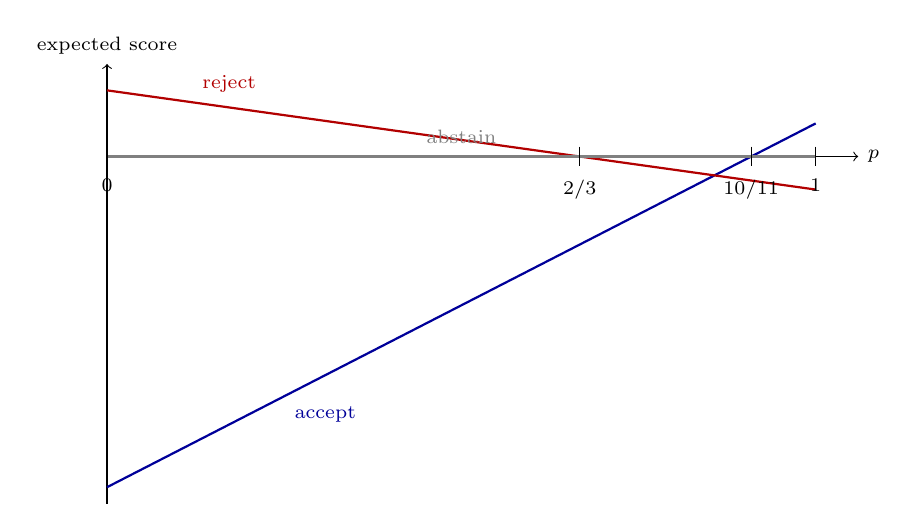
\begin{tikzpicture}[x=9cm,y=0.42cm,font=\small]
  \draw[->] (0,0) -- (1.06,0) node[right,font=\scriptsize] {$p$};
  \draw[->] (0,-10.5) -- (0,2.8) node[above,font=\scriptsize] {expected score};
  \draw[thick,blue!60!black]  (0,-10) -- (1,1)  node[pos=0.25,below right,font=\scriptsize] {accept};
  \draw[thick,red!70!black]   (0,2)   -- (1,-1) node[pos=0.12,above right,font=\scriptsize] {reject};
  \draw[thick,gray] (0,0) -- (1,0);
  \node[gray,font=\scriptsize,above] at (0.5,0.1) {abstain};
  \foreach \x/\l in {0/0, 0.667/{2/3}, 0.909/{10/11}, 1/1} {
    \draw (\x,0.3) -- (\x,-0.3);
    \node[font=\scriptsize,below] at (\x,-0.4) {$\l$};
  }
  \draw[dashed] (0.667,0) -- (0.667,-0.3);
  \draw[dashed] (0.909,0) -- (0.909,0.3);
\end{tikzpicture}
\caption{Expected score of accepting, rejecting, and abstaining as a function of the probability $p$ that the proof is valid, under the ProoVer 2026 scoring scheme. Accepting beats abstaining only for $p>10/11$, rejecting only for $p<2/3$.}
\label{fig:expected-score}
\end{figure}

\subsection{Functional Requirements}
\label{subsec:req-functional}

Table~\ref{tab:fr} lists the functional requirements.
Each requirement has an identifier that is used for traceability in Section~\ref{subsec:req-traceability} and in the evaluation.

\begin{table}[t]
\centering
\small
\caption{Functional requirements.}
\label{tab:fr}
\begin{tabular}{@{}l p{0.82\linewidth}@{}}
\toprule
ID & Requirement \\
\midrule
FR1 & Parse FOF problem and proof files, including roles, \texttt{file(\dots)} sources, \texttt{inference(\dots)} annotations with status, parents, \texttt{new\_symbols}, and \texttt{skolemize} information. \\
FR2 & Check that each \texttt{axiom} and \texttt{conjecture} in the proof is alpha-equivalent to the formula of the cited problem file and role. \\
FR3 & Check that the \texttt{negated\_conjecture} step has status \texttt{cth}, has a \texttt{conjecture} as parent, and its formula is the negation of that conjecture. \\
FR4 & Check that all cited parents exist and that the dependency graph is acyclic. \\
FR5 & Check that the \texttt{conjecture} is not used as a premise by any step other than the negation step. \\
FR6 & Check Skolemization steps: status \texttt{esa}, exactly one new Skolem symbol, a Skolem term that depends exactly on the universal variables in scope, a conclusion that results from replacing the eliminated variable by this term, and freshness of the symbol with respect to the problem and earlier steps. \\
FR7 & Check each remaining inference step with a rule-specific checker whenever one exists (structural, propositional, quantifier, junction, clausal, and equational rules). \\
FR8 & For steps without a rule-specific checker, or where a syntactic check fails on a known rule, delegate the step to an external ATP, but only if its status is \texttt{thm} or \texttt{cth} and only with the step's premises. \\
FR9 & Check that the derivation ends in \texttt{\$false}. \\
FR10 & Produce one of three verdicts per proof: verified, failed, or uncertain. \\
FR11 & Report, for each failing or uncertain step, its name, the rule, and a human-readable reason. \\
\bottomrule
\end{tabular}
\end{table}

% CODE (Stand Repo): FR9 ist NICHT als globale Prüfung implementiert (kein Check auf $false am Ende; TST036 st01_no_false testen).
% CODE (Stand Repo): FR10: validate_step_with_atp liefert bereits dreiwertig (True/False/"unknown"), main.py faltet "unknown" aber in Issues -> VerifiedBad;
%   Worker-Fehler -> VerifiedBad; nur Timeout -> "Timeout". Dreiwertiges Verdikt muss in main.py noch umgesetzt werden.

\subsection{Non-Functional Requirements}
\label{subsec:req-nonfunctional}

\begin{table}[t]
\centering
\small
\caption{Non-functional requirements.}
\label{tab:nfr}
\begin{tabular}{@{}l p{0.82\linewidth}@{}}
\toprule
ID & Requirement \\
\midrule
NFR1 & \textbf{Soundness (fail-closed).} A proof is verified only if every step has been positively validated. Missing tools, tool errors, unparsable output, and unknown rules never lead to acceptance. \\
NFR2 & \textbf{Time.} A proof must be processed within the 30-second wall-clock limit, including proofs with several thousand steps. The checker enforces its own limit and then abstains. \\
NFR3 & \textbf{Robustness.} Malformed input, deeply nested formulas, and unexpected annotations must not crash the verifier or lead to an unjustified verdict. \\
NFR4 & \textbf{Determinism.} The verdict does not depend on process scheduling or on the order of independent checks. \\
NFR5 & \textbf{Diagnostics.} Every failure is traceable to a step and a reason (FR11). \\
NFR6 & \textbf{Extensibility.} A new rule can be added without modifying the other checkers. \\
NFR7 & \textbf{Testability.} Each checker is a pure function of the proof model and can be tested in isolation; the test suite reaches a coverage of at least 85\,\%. \\
NFR8 & \textbf{Portability.} Python~3.12 and the parser library \texttt{lark} suffice for the core; an ATP is configured through environment variables and is optional. \\
\bottomrule
\end{tabular}
\end{table}

\subsection{Traceability}
\label{subsec:req-traceability}

Table~\ref{tab:trace} shows which module implements each requirement and which test files exercise it.
It is the basis for the claim that the requirements are covered and is revisited in Chapter~\ref{sec:evaluation}.

\begin{table}[t]
\centering
\small
\caption{Traceability from requirements to modules and tests.}
\label{tab:trace}
\begin{tabular}{@{}l p{0.38\linewidth} p{0.38\linewidth}@{}}
\toprule
Requirement & Module & Tests \\
\midrule
FR1 & \texttt{parser/} & \texttt{test\_parser}, \texttt{test\_parser\_transformer}, \texttt{test\_ast\_nodes} \\
FR2 & \texttt{file\_dir}, \texttt{alpha\_eq} & \texttt{test\_file\_dir}, \texttt{test\_alpha\_equivalence} \\
FR3 & \texttt{negated\_conjecture\_checker} & \texttt{test\_negated\_conjecture\_checker} \\
FR4, FR5 & \texttt{dependency\_checker} & \texttt{test\_dependency\_checker} \\
FR6 & \texttt{skolem\_checker} & \texttt{test\_skolem\_checker} \\
FR7 & \texttt{structural\_}, \texttt{propositional\_}, \texttt{junction\_}, \texttt{clausal\_}, \texttt{instantiate\_}, \texttt{existential\_gen\_checker} & matching \texttt{test\_*} files \\
FR8 & \texttt{external\_atp\_checker} & \texttt{test\_unchecked\_inference\_rules} \\
FR9--FR11 & \texttt{main.py} (\texttt{check\_proof\_file}, \texttt{report\_proof\_check}) & \texttt{test\_proof\_checker\_summary}, \texttt{test\_main\_atp\_tristate} \\
NFR2 & \texttt{main.py} (worker process), \texttt{deep\_recursion} & timing measurements (Chapter~\ref{sec:evaluation}) \\
NFR1, NFR3 & all & \texttt{test\_mutation\_fuzzing}, \texttt{test\_advanced\_edge\_cases} \\
NFR7 & CI configuration & coverage gate in the CI workflow \\
\bottomrule
\end{tabular}
\end{table}